\section*{\textbf{Social Relations Model: Additive Part of AME}}

The dependencies that tend to develop in relational data can be more easily understood when we move away from stacking dyads on top of one another and turn instead to a matrix design as illustrated in Table~\ref{tab:netDesign}. Operationally, this type of data structure is represented as a $n \times n$ matrix, $\mathbf{Y}$, where the diagonals are typically undefined. The $ij^{th}$ entry defines the relationship sent from $i$ to $j$ and can be continuous or discrete. Relations between actors in a network setting at times does not involve senders and receivers. Networks such as these are referred to as undirected and all the relations between actors are symmetric, meaning $y_{ij}=y_{ji}$.

The most common type of dependency that arises in networks are first-order, or nodal dependencies, and these point to the fact that we typically find significant heterogeneity in activity levels across nodes. The implication of this across-node heterogeneity is within-node homogeneity of ties, meaning that values across a row, say $\{y_{ij},y_{ik},y_{il}\}$, will be more similar to each other than other values in the adjacency matrix because each of these values has a common sender $i$. This type of dependency manifests in cases where sender $i$ tends to be more active or less active in the network than other senders. Similarly, while some actors may be more active in sending ties to others in the network, we might also observe that others are more popular targets, this would manifest in observations down a column, $\{y_{ji},y_{ki},y_{li}\}$, being more similar. Last, we might also find that actors who are more likely to send ties in a network are also more likely to receive them, meaning that the row and column means of an adjacency matrix may be correlated. Another ubiquitous type of structural interdependency is reciprocity. This is a second-order, or dyadic, dependency relevant only to directed datasets, and asserts that values of $y_{ij}$ and $y_{ji}$ may be statistically dependent. The prevalence of these types of potential interactions within directed dyadic data also complicates the basic assumption of observational independence.\footnote{In the Appendix, we include a lengthier discussion on the limitations of studying relational data via the typical GLM framework.}

The relevance of modeling first- and second-order dependencies has long been recognized within fields such as psychology. In 1979, Warner et al. developed the social relations model (SRM), a type of ANOVA decomposition technique, that facilitates this undertaking \cite{warner:etal:1979}. The SRM is of particular note as it provides the error structure for the additive effects component of the AME framework that we introduce here. The goal of the SRM is to decompose the variance of observations in an adjacency matrix in terms of heterogeneity across row means (out-degree), heterogeneity along column means (in-degree), correlation between row and column means, and correlations within dyads. Wong and Li \& Loken and provide a random effects representation of the SRM \cite{wong:1982,li:loken:2002}:

\begin{align}
\begin{aligned}
	y_{ij} &= \mu + e_{ij} \\
	e_{ij} &= a_{i} + b_{j} + \epsilon_{ij} \\
	\{ (a_{1}, b_{1}), \ldots, (a_{n}, b_{n}) \} &\simiid N(0,\Sigma_{ab}) \\ 
	\{ (\epsilon_{ij}, \epsilon_{ji}) : \; i \neq j\} &\simiid N(0,\Sigma_{\epsilon}), \text{ where } \\
	\Sigma_{ab} = \begin{pmatrix} \sigma_{a}^{2} & \sigma_{ab} \\ \sigma_{ab} & \sigma_{b}^2   \end{pmatrix} \;\;\;\;\; &\Sigma_{\epsilon} = \sigma_{\epsilon}^{2} \begin{pmatrix} 1 & \rho \\ \rho & 1  \end{pmatrix} .
\label{eqn:srmCov}
\end{aligned}
\end{align}

In the above, $\mu$ provides a baseline measure of the density mean of a network, and $e_{ij}$ represents residual variation. The residual variation decomposes into parts: a row/sender effect ($a_{i}$), a column/receiver effect ($b_{j}$), and a within-dyad effect ($\epsilon_{ij}$). The row and column effects are modeled jointly to account for correlation in how active an actor is in sending and receiving ties. Heterogeneity in the row and column means is captured by $\sigma_{a}^{2}$ and $\sigma_{b}^{2}$, respectively, and $\sigma_{ab}$ describes the linear relationship between these two effects (i.e., whether actors who send  a lot of ties also receive  a lot of ties). Beyond these first-order dependencies, second-order dependencies are described by $\sigma_{\epsilon}^{2}$ and a within dyad correlation, or reciprocity, parameter $\rho$. 

The SRM covariance structure described in Equation~\ref{eqn:srmCov} can be incorporated into the systematic component of a GLM framework to produce the social relations regression model (SRRM): $\bm\beta^{\top} \mathbf{X}_{ij} + a_{i} + b_{j} + \epsilon_{ij}$, where $ \bm\beta^{\top} \mathbf{X}_{ij}$ accommodates the inclusion of dyadic, sender, and receiver covariates. The SRRM approach incorporates row, column, and within-dyad dependence in way that is widely used and understood by applied researchers: a regression framework and additive random effects to accommodate variances and covariances often seen in relational data. Furthermore, this  handles a diversity of outcome distributions. In the case of binary data, this can be done by utilizing a random effects logistic (or probit) latent variable representation.

\section*{Latent Factor Model: Multiplicative Part of AME}

Missing from the framework provided by the SRM is an accounting of third-order dependence patterns that can arise in relational data. A third-order dependency is defined as the dependency between triads, not dyads. The ubiquity of third-order effects in relational datasets can arise from the presence of some set of shared attributes between nodes that affects their probability of interacting with one another. Another reason why we may see the emergence of third-order effects is the ``sociology'' explanation: that individuals want to close triads because this is putatively a more stable or preferable social situation (\citealt{wasserman:faust:1994}).

For example, one finding from the gravity model of trade is that neighboring countries are more likely to trade with one another; in this case, the shared attribute is simply geographic proximity. A finding common in the political economy literature is that democracies are more likely to form trade agreements with one another, and the shared attribute here is a country's political system. Both geographic proximity and a country's political system are examples of homophily, which captures the idea that the relationships between actors with similar characteristics in a network are likely to be stronger than nodes with different characteristics. Homophily can be used to explain the emergence of patterns such as transitivity (``a friend of a friend is a friend'') and balance (``an enemy of a friend is an enemy''). 

A binary network where actors tend to form ties with others based on some set of shared characteristics often leads to a network graph with a high number of ``transitive triads'' in which  sets of actors $\{i,j,k\}$ are each linked to one another. The left-most plot in Figure~\ref{fig:homphStochEquivNet} provides a representation of a network that exhibits this type of pattern. The relevant implication of this when it comes to conducting statistical inference is that--unless we are able to specify the list of exogenous variable that may explain this prevalence of triads--the probability of $j$ and $k$ forming a tie is not independent of the ties that already exist between those actors and $i$.

\begin{figure}[ht]
	\centering
	\caption{Graph on the left is a representation of an undirected network that exhibits a high degree of homophily, while on the right we show an undirected network that exhibits stochastic equivalence.}	
	\begin{tabular}{lcr}
	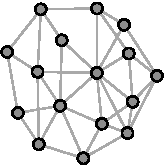
\includegraphics[width=.33\textwidth]{homophNet} & \hspace{2cm} &
	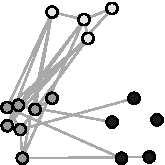
\includegraphics[width=.33\textwidth]{stochEquivNet}	
	\end{tabular}
	\label{fig:homphStochEquivNet}
\end{figure}

Another third-order dependence pattern that cannot be accounted for in the additive effects framework is stochastic equivalence. A pair of actors $ij$ are stochastically equivalent if the probability of $i$ relating to, and being related to, by every other actor is the same as the probability for $j$. This refers to the idea that there will be groups of nodes in a network with similar relational patterns. The occurrence of a dependence pattern such as this is not uncommon in the social science applications. Recent work estimates a stochastic equivalence structure to explain the formation of preferential trade agreements (PTAs) between countries \cite{manger:etal:2012}. Specifically, they suggest that PTA formation is related to differences in per capita income levels between countries. Countries falling into high, middle, and low income per capita levels will have patterns of PTA formation that are determined by the groups into which they fall. Such a structure is represented in the right-most panel of Figure~\ref{fig:homphStochEquivNet}, here the lightly shaded group of nodes at the top can represent high-income countries, nodes on the bottom-left middle-income, and the darkest shade of nodes low-income countries. The behavior of actors in a network can at times be governed by group level dynamics, and failing to account for such dynamics leaves potentially important parts of the data generating process ignored.

To account for third-order dependence patterns within the context of the SRRM we turn to latent variable models, which have become a popular approach for modeling relational data in fields as diverse as biology to computer science to the social sciences. These models assumes that relationships between nodes are mediated by a small number ($K$) of node-specific unobserved latent variables. One reason for their increased usage is that they enable researchers to capture and visualize third-order dependencies in a way that other approaches are not able to replicate.

A number of latent variable approaches have been developed to represent third-order dependencies in relational data, we focus on two here: the the latent space model (LSM) and the latent factor model (LFM).\footnote{An alternative approach with a similar latent variable formulation is known as the stochastic block model \citep{nowicki:snijders:2001}. } For the sake of exposition, we consider the case where relations are symmetric to describe the differences between these approaches. These approaches can be incorporated into the framework that we have been constructing through the inclusion of an additional term, $\alpha(\mu_{i}, \mu_{j})$, that captures latent third order characteristics of a network. General definitions for how $\alpha(u_{i}, u_{j})$ are defined for these latent variable models are shown in Equations~\ref{eqn:latAlpha}. One other point of note about these approaches is that researchers have to specify a value for $K$.\footnote{In the case of both the latent space and factor models, a value of $K$ equal to two or three is typically large enough to account for third-order dependencies in relational data.} These two approaches are described below:

\begin{align}
\begin{aligned}
\text{Latent space model} \\
	&\alpha(\textbf{u}_{i}, \textbf{u}_{j}) = -|\textbf{u}_{i} - \textbf{u}_{j}| \\
	&\textbf{u}_{i} \in \mathbb{R}^{K}, \; i \in \{1, \ldots, n \} \\
\text{Latent factor model} \\
	&\alpha(\textbf{u}_{i}, \textbf{u}_{j}) = \textbf{u}_{i}^{\top} \Lambda \textbf{u}_{j} \\
	&\textbf{u}_{i} \in \mathbb{R}^{K}, \; i \in \{1, \ldots, n \} \\
	&\Lambda \text{ a } K \times K \text{ diagonal matrix}
\label{eqn:latAlpha}
\end{aligned}
\end{align}

In the LSM approach, each node $i$ has some unknown latent position in $K$ dimensional space, $\textbf{u}_{i} \in \mathbb{R}^{K}$, and the probability of a tie between a pair $ij$ is a function of the negative Euclidean distance between them: $-|\textbf{u}_{i} - \textbf{u}_{j}|$. Because latent distances for a triple of actors obey the triangle inequality, this formulation models the tendencies toward homophily commonly found in social networks. This approach is implemented in the \pkg{latentnet} which is part of the \pkg{statnet} $\sf{R}$ package \cite{krivitsky:handcock:2015}. However, this approach also comes with an important shortcoming: it confounds stochastic equivalence and homophily. Consider two nodes $i$ and $j$ that are proximate to one another in $K$ dimensional Euclidean space, this suggests not only that $|\textbf{u}_{i} - \textbf{u}_{j}|$ is small but also that $|\textbf{u}_{i} - \textbf{u}_{l}| \approx |\textbf{u}_{j} - \textbf{u}_{l}|$, the result being that nodes $i$ and $j$ will by construction assumed to possess the same relational patterns with other actors such as $l$ (i.e., that they are stochastically equivalent). Thus LSMs confound strong ties with stochastic equivalence. This approach cannot adequately model data with many ties between nodes that have different network roles.

This is problematic as real-world networks exhibit varying degrees of stochastic equivalence and homophily. In these situations, using the LSM would end up representing only a part of the network structure. In the latent factor model, each actor has an unobserved vector of characteristics, $\textbf{u}_{i} = \{u_{i,1}, \ldots, u_{i,K} \}$, which describe their behavior as an actor in the network. The probability of a tie from $i$ to $j$ depends on the extent to which $\textbf{u}_{i}$ and $\textbf{u}_{j}$ are ``similar'' (i.e., point in the same direction) and on whether the entries of $\Lambda$ are greater or less than zero.

More specifically, the similarity in the latent factors, $\textbf{u}_{i} \approx \textbf{u}_{j}$, corresponds to how stochastically equivalent a pair of actors are and the eigenvalue determines whether the network exhibits positive or negative homophily. For example, say that we estimate a rank-one latent factor model (i.e., $K=1$), in this case $\textbf{u}_{i}$ is represented by a scalar $u_{i,1}$, similarly, $\textbf{u}_{j}=u_{j,1}$, and $\Lambda$ will have just one diagonal element $\lambda$. The average effect this will have on $y_{ij}$ is simply $\lambda \times u_{i} \times u_{j}$, where a positive value of $\lambda>0$ indicates homophily and $\lambda<0$ heterophily. This approach can represent both varying degrees of homophily and stochastic equivalence. In the directed version of this approach, we use the singular value decomposition, here actors in the network have a vector of latent characteristics to describe their behavior as a sender, denoted by $\textbf{u}$, and as a receiver, $\textbf{v}$: $\textbf{u}_{i}, \textbf{v}_{j} \in \mathbb{R}^{K}$. This can alter the probability of an interaction between $ij$ additively: $\textbf{u}_{i}^{\top} \textbf{D} \textbf{v}_{j}$, where $\textbf{D}$ is a $K \times K$ diagonal matrix.

Both the latent space and factor models are ``conditional independence models'' in that they assume that ties are conditionally independent given all of the observed predictors and unknown node-specific parameters: $p( Y | X , U ) = \prod_{i<j} p( y_{i,j}  | x_{i,j} , u_i , u_j)$. Typical parametric models of this form relate $y_{i,j}$ to $(x_{i,j},u_i,u_j)$ via some sort of link function:

\begin{align*}
	p(y_{i,j} | x_{i,j}, u_i , u_j ) & = f( y_{i,j} : \eta_{i,j} ) \\
	\eta_{i,j} &= \beta^\top x_{i,j} + \alpha(\textbf{u}_{i}, \textbf{u}_{j}).
\end{align*}

The structure of $\alpha(\textbf{u}_{i}, \textbf{u}_{j})$ can result in very different interpretations for any estimates of the regression coefficients $\beta$. For example, suppose the latent effects $\{ u_1,\ldots, u_n\}$ are near zero on average (if not, their mean can be absorbed into an intercept parameter and row and column additive effects). Under the LFM, the average value of $\alpha(\textbf{u}_{i}, \textbf{u}_{j}) = \textbf{u}_{i}^{\top} \Lambda \textbf{u}_{j}$ will be near zero and so we have

\begin{align*}
	\eta_{i,j} & =  \beta^\top x_{i,j} + \textbf{u}_{i}^{\top} \Lambda \textbf{u}_{j} \\
	\bar \eta & \approx  \beta^\top \bar x.
\end{align*}

The implication of this is that the values of $\beta$ can be interpreted as yielding the ``average'' value of $\eta_{i,j}$. On the other hand, under the LSM

\begin{align*}
	\eta_{i,j} & =  \beta^\top x_{i,j} - |\textbf{u}_{i} - \textbf{u}_{j}|  \\
	\bar \eta & \approx  \beta^\top \bar x - \overline{ |\textbf{u}_{i} - \textbf{u}_{j}| } <  \beta^\top \bar x .
\end{align*}

In this case, $\beta^\top \bar x$ does not represent an ``average'' value of the predictor $\eta_{i,j}$, it represents a maximal value as if all actors were zero distance from each other in the latent social space. For example, consider the simplest case of a normally distributed network  outcome with an identity link. In this case,

\begin{align*}
	y_{i,j} & = \beta^\top x_{i,j} + \alpha(\textbf{u}_{i}, \textbf{u}_{j}) + \epsilon_{i,j} \\
	\bar y & \approx \beta^\top \bar x + \overline{ \alpha(\textbf{u}_{i}, \textbf{u}_{j}) }   .
\end{align*}

Under the LSM, $\bar y \approx \beta^\top \bar x + \overline{ |\textbf{u}_{i} - \textbf{u}_{j}|  } < \beta^\top \bar x$, and so we no longer can interpret $\beta$ as representing the linear relationship between $y$ and $x$. Instead, it may be thought of as describing some sort of average hypothetical ``maximal'' relationship between $y_{i,j}$ and $x_{i,j}$.

Thus the LFM provides two important benefits. First, we are able to capture a wider assortment of dependence patterns that arise in relational data, and, second, parameter interpretation is more straightforward. The AME approach considers the regression model shown in Equation~\ref{eqn:ame}:

\begin{align}
\begin{aligned}
	y_{ij} &= g(\theta_{ij}) \\
	&\theta_{ij} = \bm\beta^{\top} \mathbf{X}_{ij} + e_{ij} \\
	&e_{ij} = a_{i} + b_{j}  + \epsilon_{ij} + \alpha(\textbf{u}_{i}, \textbf{v}_{j}) \text{  , where } \\
	&\qquad \alpha(\textbf{u}_{i}, \textbf{v}_{j}) = \textbf{u}_{i}^{\top} \textbf{D} \textbf{v}_{j} = \sum_{k \in K} d_{k} u_{ik} v_{jk}. \\
\label{eqn:ame}
\end{aligned}
\end{align}

Using this framework, we are able to model the dyadic observations as conditionally independent given $\bm\theta$, where $\bm\theta$ depends on the the unobserved random effects, $\mathbf{e}$. $\mathbf{e}$ is then modeled to account for the potential first, second, and third-order dependencies that we have discussed. As described in Equation~\ref{eqn:srmCov}, $a_{i} + b_{j}  + \epsilon_{ij}$, are the additive random effects in this framework and account for sender, receiver, and within-dyad dependence. The multiplicative effects, $\textbf{u}_{i}^{\top} \textbf{D} \textbf{v}_{j}$, are used to capture higher-order dependence patterns that are left over in $\bm\theta$ after accounting for any known covariate information. %A Bayesian procedure in which parameters are iteratively updated using a Gibbs sampler is available in an $\sf{R}$ package.%\footnote{The set of parameters that are estimated in the model from the observed data, $\{\mathbf{Y}, \mathbf{X}\}$, are: latent Gaussian variables ($\bm\theta$); nodal and/or dyadic regression coefficients ($\bm\beta$); additive nodal random effects ($\{(a_{i},b_{i})\} \in \{i=1, \ldots, n \}$); network covariance ($\Sigma_{ab},\, \Sigma_{\epsilon}$); multiplicative effects ($\mathbf{U}$, $\mathbf{V}$, and $\mathbf{D}$).}

In the following section we undertake a comparison of the latent space model, ERGM, and the AME model. In doing so, we are able to compare and contrast these various approaches.
